\documentclass[border=10pt, tikz]{standalone}
\usepackage[T1]{fontenc}
\usepackage{helvet}
\renewcommand{\familydefault}{\sfdefault}
\usepackage{amsmath, amssymb}
\usetikzlibrary{arrows.meta, positioning, calc, backgrounds, fit}

\definecolor{slateDark}{HTML}{0F172A}
\definecolor{slateText}{HTML}{334155}
\definecolor{slateMuted}{HTML}{64748B}
\definecolor{slateBorder}{HTML}{CBD5E1}
\definecolor{slateBg}{HTML}{F8FAFC}

\definecolor{redDark}{HTML}{991B1B}
\definecolor{redMain}{HTML}{DC2626}
\definecolor{redBg}{HTML}{FEF2F2}

\definecolor{blueDark}{HTML}{0369A1}
\definecolor{blueMain}{HTML}{0284C7}
\definecolor{blueBg}{HTML}{F0F9FF}

\definecolor{purpleDark}{HTML}{5B21B6}
\definecolor{purpleMain}{HTML}{7C3AED}
\definecolor{purpleBg}{HTML}{F5F3FF}

\begin{document}
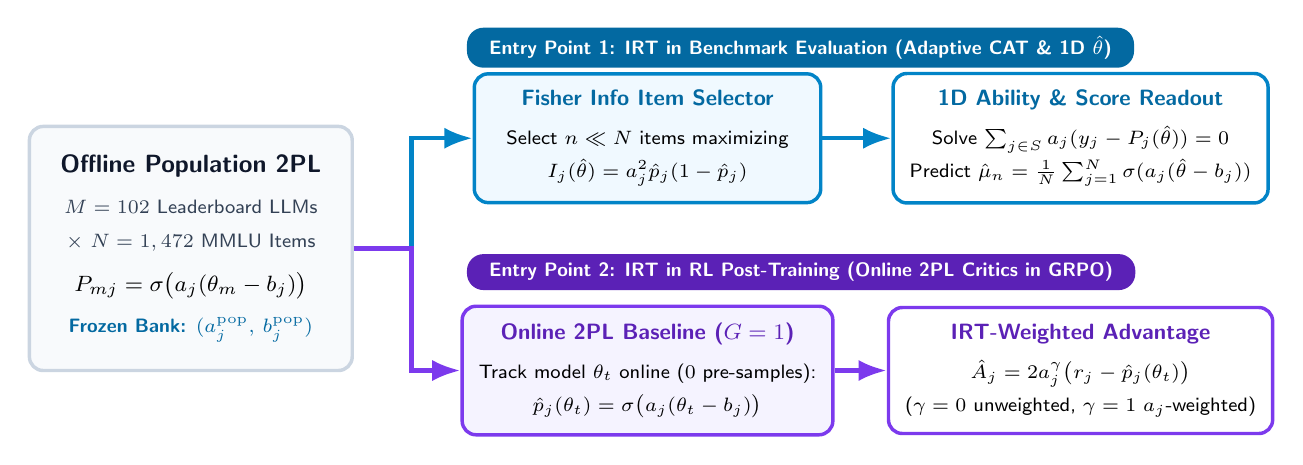
\begin{tikzpicture}[
    >=Latex,
    font=\sffamily,
    box/.style={
        rectangle,
        rounded corners=5pt,
        draw=#1,
        line width=1.25pt,
        fill=white,
        align=center,
        inner sep=6pt
    },
    pill/.style={
        rectangle,
        rounded corners=6pt,
        fill=#1,
        text=white,
        font=\sffamily\bfseries\scriptsize,
        inner xsep=8pt,
        inner ysep=3pt
    },
    arrow/.style={
        ->,
        line width=1.6pt,
        color=#1
    }
]

% Left: Offline Population Calibration
\node[box=slateBorder, fill=slateBg, minimum width=4.1cm, minimum height=3.1cm] (pop) at (-7.0, -0.05) {
    \textbf{\small\color{slateDark} Offline Population 2PL}\\[3pt]
    {\scriptsize\color{slateText} $M = 102$ Leaderboard LLMs}\\
    {\scriptsize\color{slateText} $\times$ $N = 1,472$ MMLU Items}\\[4pt]
    {\footnotesize $P_{mj} = \sigma\big(a_j(\theta_m - b_j)\big)$}\\[3pt]
    {\scriptsize\color{blueDark} \textbf{Frozen Bank: $(a_j^{\mathrm{pop}}, \, b_j^{\mathrm{pop}})$}}
};

% Top Branch: Entry Point 1 (Evaluation / CAT)
\node[pill=blueDark, anchor=west] at (-3.5, 2.5) {Entry Point 1: IRT in Benchmark Evaluation (Adaptive CAT \& 1D $\hat{\theta}$)};

\node[box=blueMain, fill=blueBg, minimum width=4.4cm, minimum height=1.35cm] (cat1) at (-1.2, 1.35) {
    \textbf{\footnotesize\color{blueDark} Fisher Info Item Selector}\\[2pt]
    {\scriptsize Select $n \ll N$ items maximizing}\\
    {\scriptsize $I_j(\hat{\theta}) = a_j^2 \hat{p}_j(1-\hat{p}_j)$}
};

\node[box=blueMain, fill=white, minimum width=4.5cm, minimum height=1.35cm] (cat2) at (4.3, 1.35) {
    \textbf{\footnotesize\color{blueDark} 1D Ability \& Score Readout}\\[2pt]
    {\scriptsize Solve $\sum_{j \in S} a_j(y_j - P_j(\hat{\theta})) = 0$}\\
    {\scriptsize Predict $\hat{\mu}_n = \frac{1}{N}\sum_{j=1}^N \sigma(a_j(\hat{\theta}-b_j))$}
};

% Bottom Branch: Entry Point 2 (RL Training / GRPO Critics)
\node[pill=purpleDark, anchor=west] at (-3.5, -0.35) {Entry Point 2: IRT in RL Post-Training (Online 2PL Critics in GRPO)};

\node[box=purpleMain, fill=purpleBg, minimum width=4.4cm, minimum height=1.45cm] (rlc1) at (-1.2, -1.6) {
    \textbf{\footnotesize\color{purpleDark} Online 2PL Baseline ($G=1$)}\\[2pt]
    {\scriptsize Track model $\theta_t$ online ($0$ pre-samples):}\\
    {\scriptsize $\hat{p}_j(\theta_t) = \sigma\big(a_j(\theta_t - b_j)\big)$}
};

\node[box=purpleMain, fill=white, minimum width=4.5cm, minimum height=1.45cm] (rlc2) at (4.3, -1.6) {
    \textbf{\footnotesize\color{purpleDark} IRT-Weighted Advantage}\\[2pt]
    {\scriptsize $\hat{A}_j = 2 a_j^\gamma \big(r_j - \hat{p}_j(\theta_t)\big)$}\\
    {\scriptsize ($\gamma=0$ unweighted, $\gamma=1$ $a_j$-weighted)}
};

% Arrows
\draw[arrow=blueMain] (pop.east) -- (-4.2, -0.05) |- (cat1.west);
\draw[arrow=blueMain] (cat1.east) -- (cat2.west);

\draw[arrow=purpleMain] (pop.east) -- (-4.2, -0.05) |- (rlc1.west);
\draw[arrow=purpleMain] (rlc1.east) -- (rlc2.west);

\end{tikzpicture}
\end{document}
